\section{Projektowanie tabel, kluczy, kluczy obcych, powiązań między tabelami, indeksów, etc. w oparciu o zdefiniowany diagram ERD;} 

%na tym etapie następuje „sprecyzowanie” struktury bazy danych wraz ze szczegółami technicznymi. Projekt bazy w języku SQL.

%\begin{figure}[!htp]
%    \centering
%    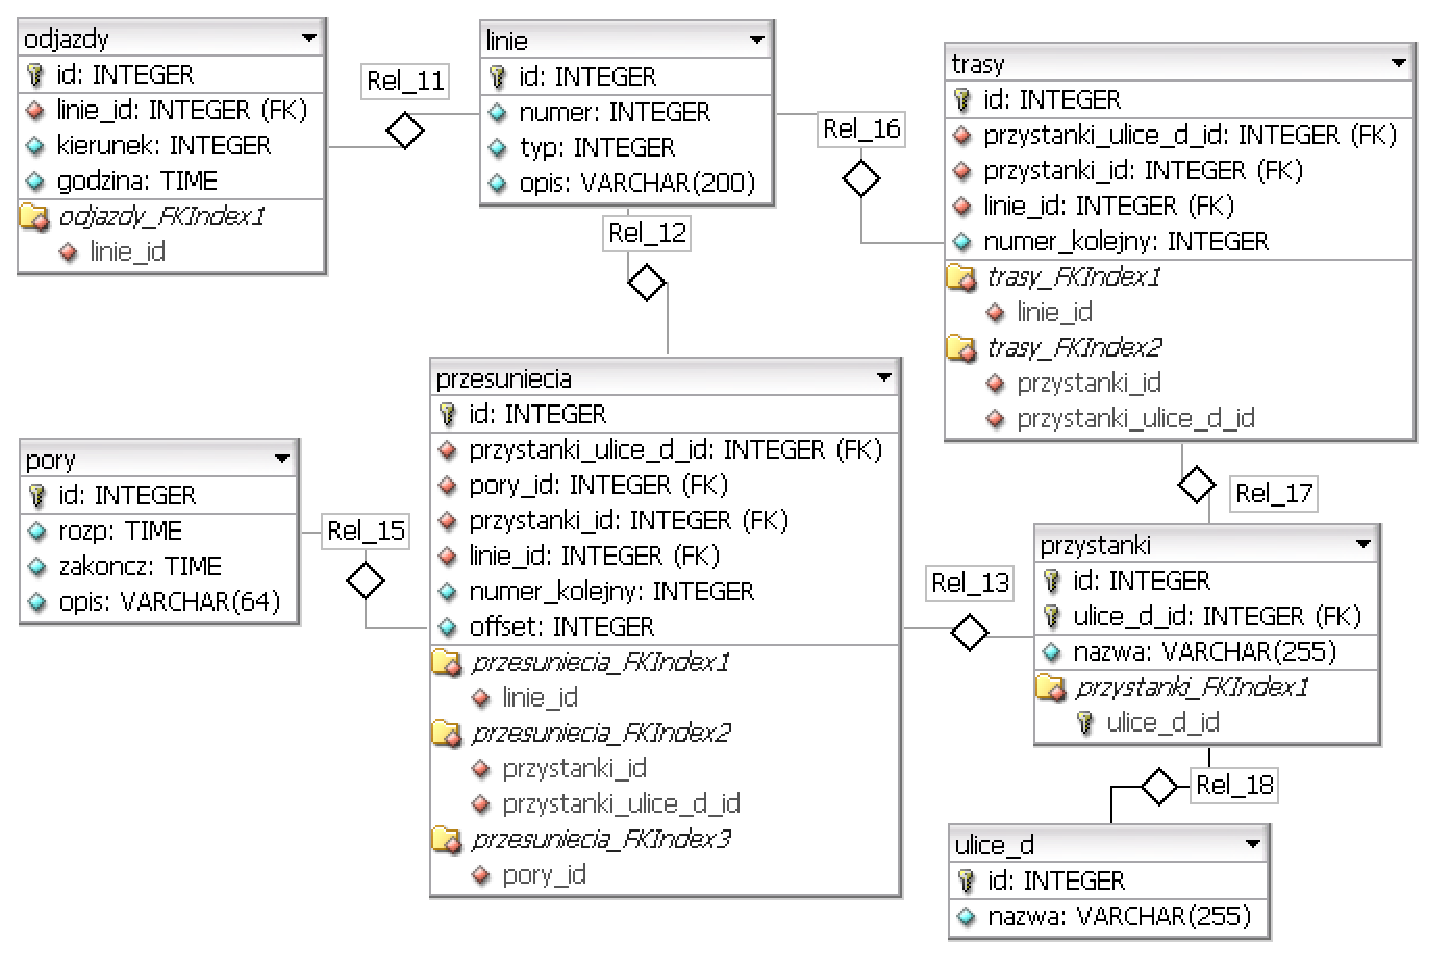
\includegraphics[width=0.75\textwidth]{./img/busag_model.eps}
%    \caption{Tabele}
%    \label{fig:tabs}
%\end{figure}

\begin{verbatim}
 CREATE TABLE linie (
    numer integer NOT NULL,
    typ integer NOT NULL,
    opis character varying(200)
);

CREATE TABLE odjazdy (
    id integer NOT NULL,
    linie_id integer NOT NULL,
    godzina time without time zone,
    kierunek bit(1) NOT NULL
);

CREATE TABLE pory (
    id integer NOT NULL,
    rozp time without time zone NOT NULL,
    zakoncz time without time zone NOT NULL,
    opis character varying(64) NOT NULL
);

CREATE TABLE przesuniecia (
    id integer NOT NULL,
    "offset" interval NOT NULL,
    trasy_id integer,
    powrotna bit(1) NOT NULL
);

CREATE TABLE przystanki (
    id integer NOT NULL,
    nazwa character varying NOT NULL,
    ulica1_id integer,
    ulica2_id integer
);

CREATE TABLE trasy (
    id integer NOT NULL,
    linie_id integer,
    przystanki_id integer,
    numer_kolejny integer
);

CREATE VIEW timetable_view AS
    SELECT odjazdy.linie_id AS linia_numer, trasy.numer_kolejny, przystanki.id AS przystanek_id, przystanki.nazwa AS przystanek, (przesuniecia."offset" + odjazdy.godzina) AS odj, odjazdy.id AS odj_id, odjazdy.kierunek FROM (((przesuniecia JOIN trasy ON ((przesuniecia.trasy_id = trasy.id))) JOIN przystanki ON ((trasy.przystanki_id = przystanki.id))) JOIN odjazdy ON ((odjazdy.linie_id = trasy.linie_id))) WHERE (odjazdy.kierunek = przesuniecia.powrotna) ORDER BY odjazdy.linie_id, trasy.numer_kolejny;


CREATE VIEW trasy_view AS
    SELECT trasy.przystanki_id, linie.numer, trasy.numer_kolejny, (SELECT przystanki.nazwa FROM przystanki WHERE (przystanki.id = trasy.przystanki_id)) AS nazwa FROM (trasy JOIN linie ON ((linie.numer = trasy.linie_id)));


ALTER TABLE ONLY linie
    ADD CONSTRAINT linie_numer_key UNIQUE (numer);

ALTER TABLE ONLY linie
    ADD CONSTRAINT linie_pkey PRIMARY KEY (numer);

ALTER TABLE ONLY odjazdy
    ADD CONSTRAINT odjazdy_pkey PRIMARY KEY (id);

ALTER TABLE ONLY pory
    ADD CONSTRAINT pory_pkey PRIMARY KEY (id);

ALTER TABLE ONLY przesuniecia
    ADD CONSTRAINT przesuniecia_pkey PRIMARY KEY (id);

ALTER TABLE ONLY przystanki
    ADD CONSTRAINT przystanki_nazwa_key UNIQUE (nazwa);

ALTER TABLE ONLY przystanki
    ADD CONSTRAINT przystanki_pkey PRIMARY KEY (id);

ALTER TABLE ONLY trasy
    ADD CONSTRAINT trasy_pkey PRIMARY KEY (id);

ALTER TABLE ONLY odjazdy
    ADD CONSTRAINT odjazdy_linie_id_fkey FOREIGN KEY (linie_id) REFERENCES linie(numer) ON UPDATE CASCADE ON DELETE CASCADE;

ALTER TABLE ONLY przesuniecia
    ADD CONSTRAINT przesuniecia_trasy_id_fkey FOREIGN KEY (trasy_id) REFERENCES trasy(id) ON UPDATE CASCADE ON DELETE CASCADE;

ALTER TABLE ONLY przystanki
    ADD CONSTRAINT przystanki_fk_id_ulica1_fkey FOREIGN KEY (ulica2_id) REFERENCES ulice_d(id);

ALTER TABLE ONLY przystanki
    ADD CONSTRAINT przystanki_fk_id_ulica2_fkey FOREIGN KEY (ulica1_id) REFERENCES ulice_d(id);

ALTER TABLE ONLY trasy
    ADD CONSTRAINT trasy_linie_id_fkey FOREIGN KEY (linie_id) REFERENCES linie(numer) ON UPDATE CASCADE ON DELETE CASCADE;

ALTER TABLE ONLY trasy
    ADD CONSTRAINT trasy_przystanki_id_fkey FOREIGN KEY (przystanki_id) REFERENCES przystanki(id) ON UPDATE CASCADE ON DELETE RESTRICT;
\end{verbatim}



